\documentclass{article}
\usepackage[T1]{fontenc}
\usepackage[utf8]{inputenc}
\usepackage{graphicx}
\graphicspath{ {./images/} }
\usepackage[french]{babel}
\usepackage{xcolor}
\usepackage{pgfplots}
\pgfplotsset{compat=1.7}
\usepackage{tikz}
\usepackage{float}
\usepackage{indentfirst}
\usetikzlibrary{arrows,shapes,positioning}
\usetikzlibrary{decorations.markings,decorations.pathmorphing,
decorations.pathreplacing}
\usetikzlibrary{calc,patterns,shapes.geometric}
\definecolor{commentgreen}{RGB}{2,112,10}
\definecolor{eminence}{RGB}{108,48,130}
\definecolor{weborange}{RGB}{255,165,0}
\definecolor{frenchplum}{RGB}{129,20,83}
\usetikzlibrary{arrows,automata}
\usepackage{listings}
\usepackage{hyperref}
\usepackage{fancyhdr}
\usepackage{algorithm}
\usepackage{algorithmic}
\hypersetup{
    colorlinks=true,
    linkcolor=black,
    filecolor=magenta,      
    urlcolor=cyan
    citecolor=green
}

\lstset {
    language=C,
    frame=tb,
    tabsize=4,
    showstringspaces=false,
    numbers=left,
    %upquote=true,
    commentstyle=\color{commentgreen},
    keywordstyle=\color{blue},
    stringstyle=\color{red},
    basicstyle=\small\ttfamily\color{blue}, % basic font setting
    emph={int,char,double,float,unsigned,void,bool},
    emphstyle={\color{blue}},
    escapechar=\&,
    % keyword highlighting
    classoffset=1, % starting new class
    otherkeywords={>,<,.,;,-,!,=,~},
    morekeywords={>,<,.,;,-,!,=,~,\&},
    keywordstyle=\color{blue},
    classoffset=0,
}

\title{Rapport de projet Racket : Hex}
\author{Auteurs : Boudroua Imad, Gauchet Augustin, Nguyen Olivier, Zghari Hicham \\ Equipe 9145 \\ Encadrants : M.Renault et M.Méaux}

\usepackage{geometry}%Marges
\geometry{left=3.5cm, right=3cm}

\begin{document}
%\maketitle
%
\includegraphics[width=\textwidth]{logo.jpg}
\thispagestyle{empty}
\begin{figure}%[ht]

\includegraphics[scale=0.6]{logo.jpg}
\end{figure}

\label{sommaire}

\begin{center}
\begin{tikzpicture}
\node[align=center,draw,thick,minimum width=\textwidth,inner sep=6mm] (titlebox)%
{\textsc{\textbf{\huge S6}}\\[\baselineskip]\textsc{\ }\\[\baselineskip]\textbf{\Huge HEX Project}\textsc{\ }\\[\baselineskip]};
\node[fill=white] (W) at (titlebox.north) {\bfseries \huge Projet};
\node (feat) at ([yshift=-9mm]titlebox.south){\bfseries \Large Boudroua Imad \ \ \ Zghari Hicham};
\node (feat) at ([yshift=-18mm]titlebox.south){\bfseries \Large \ Nguyen Olivier \ \ \ Gauchet Augustin};
\node (feat) at ([yshift=-27mm]titlebox.south){\bfseries \Large Equipe 9145};
\node (feat) at ([yshift=-60mm]titlebox.south){\bfseries \Large \ Encadrants : M.Renault et M.Méaux};
\end{tikzpicture}
\end{center}

\newpage

\pagestyle{fancy}
\fancyhf{}
\lfoot{Equipe 9145}
\rfoot{Page \thepage/\pageref{LastPage}}
\renewcommand{\headrulewidth}{0pt}
\renewcommand{\footrulewidth}{0pt}

\tableofcontents
\newpage

\section{Introduction et analyse du projet}
\subsection{Contexte}
Dans le cadre du second projet de programmation en première année d'informatique à l'ENSEIRB-MATMECA, nous avons eu à coder le jeu \textbf{Hex}, à l'aide du langage de programmation impérative \textbf{C}. Ce rapport va permettre d'expliquer les démarches que notre groupe a effectuées pour mener ce projet.

\subsection{Problématique}
\textbf{Hex} est un jeu qui se joue à deux joueurs où chacun incarne une couleur et joue à tour de rôle. Pour gagner, le joueur doit relier deux bords de sa couleur par une chaîne continue de pions lui appartenant. Une des particularités de ce jeu est de pouvoir se jouer sur un plateau de taille et de forme variables. Ainsi le but de notre projet sera de modéliser ce jeu sur des plateaux hexagonaux, triangulaires ou même carrés et de créer des algorithmes pouvant jouer efficacement au jeu.

\subsection{Cadre de travail}
A cause de la pandémie de Coronavirus, nous avons dû travailler chez nous, certains en SSH et d'autres en machines virtuelles. Les différences de configuration et le manque de maîtrise du SSH ont notamment été un frein au développement du projet. 

%\subsection{Bibliothèques utilisées}
%\subsubsection{La bibliothèque GSL}
%Le graphe a été représenté par des matrices d'appartenance, crées grâce à la bibliothèque GSL.

\section{Mise en oeuvre technique}

\subsection{Le serveur}
\subsubsection{Chargement des joueurs}
Le serveur charge dynamiquement les joueurs (clients) passés en ligne de commande de manière dynamique. Il permet de faire jouer des clients de manière indépendante. Le fait d'isoler le serveur de la partie client assure d'une part un jeu sans triche, et d'autre part cela permet de moduler les joueurs. Lorsqu'un des clients essaie de jouer sur une case interdite par les règles, il perd instantanément la partie. 
\subsubsection{Organisation du jeu}

 Afin de faciliter la manipulation des joueurs, nous avons crée une structure \lstinline{player_server} indépendante de celle implémentée dans la partie client. Celle-ci contient les principaux pointeurs de fonctions nécessaires au fonctionnement du jeu. Son utilisation nous a permis d'éviter une duplication de code et d'organiser notre serveur. 
 \subsubsection{Boucle de jeu}
 Tout d'abord, les deux joueurs en entrée du programme sont initialisés. Ensuite, un des deux propose un premier coup. Si l'adversaire accepte la proposition, leur couleur est affectée. La fonction \lstinline{compute_next_player} décide qui va prendre la main en fonction du coup précédent. Le jeu se termine lorsque l'un des deux joueurs gagne.
 \subsubsection{Affichage du jeu}

 Pour l'affichage du jeu, nous avons procédé selon deux manières : La première consiste à utiliser la fonction \lstinline{print_graph} qui affiche le jeu sur le terminal. Pour ce qui est de la deuxième méthode, nous avons écrit les données de jeu produites dans le serveur directement dans un fichier java-script dans lequel nous avons traité ces informations.


\subsection{Le joueur}
Les clients sont codés indépendemment et sont sauvegardés dans des bibliothèques dynamiques pour pouvoir les confronter à d'autres joueurs et dans d'autres serveurs que les nôtres. Chacun de nos clients est composé d'une structure \textit{player}, cette dernière contenant notamment une sauvegarde du plateau de jeu, un champ désignant leur couleur et des pointeurs de fonctions.

\subsection{Graphes et plateau de jeu}

\subsubsection{Structure des graphes}

Dans ce projet, le plateau de jeu est représenté par la structure \lstinline{graph_t}. Cette structure contient un nombre de sommets $num\_vertices$ (noté $n$ par la suite dans un souci de concision), une matrice d'adjacence $t$ de taille $n*n$ matérialisant les liaisons entre les sommets, et d'une matrice $o$ de taille $2*n$ qui définit la coloration des cases. Chaque ligne de cette matrice correspond à une couleur, et si le i\up{eme} élément de cette ligne est non nul, c'est que la case correspondante appartient au joueur de cette couleur.

Les matrices sont implémentées en utilisant les matrices creuses de la bibliothèque \emph{GNU Scientific Library}. Ce choix permet de minimiser l'utilisation de la mémoire lorsqu'on a affaire à des matrices dont la plupart des éléments sont nuls.

Il a donc été nécessaire de réaliser les fonctions permettant d'initialiser et d'afficher le plateau de jeu en fonction de sa taille et de sa forme (hexagonale, carrée ou triangulaire). Pour initialiser les cases du plateau initial, les éléments de la matrice o sont d'abord initialisés à $0$. Ensuite pour chaque couleur, les sommets appartenant à un bord sont mis à 2 pour cette couleur et ceux du bord d'en face à 3. Cela permet par la suite de pouvoir différencier les bords entre eux, ainsi que des autres cases qui auront pour valeur soit 0, soit 1.


\subsubsection{Condition de victoire et complexité}

Pour assurer le bon déroulement du jeu, il est nécessaire de pouvoir vérifier si un joueur a gagné. Pour ce faire, nous avons dans un premier temps implémenté une pile (une file aurait aussi fait l'affaire).

La pile est implémentée comme un tableau de taille et de capacité connues. On peut donc dépiler en temps constant en diminuant \lstinline{size}. En ce qui concerne l'empilement, on empile en temps constant si la taille est strictement inférieure à la capacité. Dans le cas contraire, il faut ré-allouer le tableau avec une taille deux fois plus grande. Cependant bien que cela signifie une complexité en temps linéaire dans le pire des cas, la complexité en temps moyenne est constante. La création ainsi que la libération de la pile se font également en temps constant.

La fonction \lstinline{is_winning} utilise cette pile pour vérifier si un joueur a gagné via un parcours en profondeur. Elle utilise également un tableau $tab$ de taille $n$ qui permet de savoir en temps constant si un sommet a été empilé auparavant. Elle commence par empiler le dernier sommet colorié. Puis, tant que la pile n'est pas vide, elle dépile pour obtenir un sommet, ensuite elle le marque comme visité dans le tableau $tab$ et empile tous les sommets adjacents de la couleur du tout premier sommet et qui n'ont pas déjà été empilés. Cet empilement se fait en temps linéaire en fonction de $n$ puisqu'on parcourt une ligne de la matrice d'adjacence. On vérifie au passage si un sommet fait partie d'un bord. Si à un moment donné les deux bords ont été visités, c'est que le joueur a gagné.

Dans le pire des cas, cette fonction visite la moitié des sommets du graphes, sa complexité en temps est donc en \textbf{O(n * n)}.

\section{Stratégies employées}

\subsection{La stratégie aléatoire}
Notre première stratégie est naïve. Elle consiste à jouer aléatoirement sur une case parmi celles qui sont possibles (les cases non colorées). En effet, les cases disponibles sont stockées dans un tableau. Ensuite, le joueur choisit aléatoirement une position parmi les valeurs valides du tableau. Cette valeur représentera son prochain coup.  
La complexité de cette stratégie est linéaire en fonction des positions disponibles sur la table du jeu.

\subsection{La stratégie du bloqueur}
Le but de cette stratégie est de bloquer l'autre joueur. En effet, les coups de l'adversaire cherchent à construire un chemin entre deux bords de la même couleur de la table de jeu, donc notre stratégie essaye de couper ce chemin en mettant un obstacle devant le dernier coup de l'adversaire.
\\

Dans l'exemple suivant, le prochain coup du joueur bloqueur (bleu) est dans la position \textbf{B}. En effet, bloquer le joueur en rouge à la position \textbf{A} revient à s'opposer à son cheminement vers son bord.
Dans le cas où le voisin de gauche de la dernière position n'est pas vide, le voisin de droite est traité.

\begin{figure}[H]
\centering
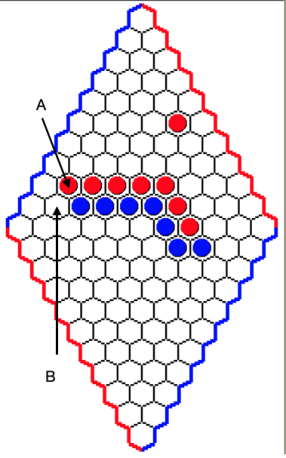
\includegraphics[scale=0.5]{1.png}
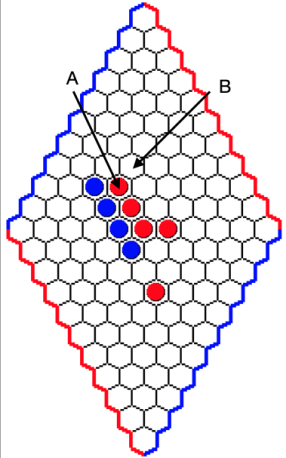
\includegraphics[scale=0.5]{2.png}
\end{figure}

Si les deux positions sont prises, les cases voisines du haut puis du bas sont traitées en prenant en compte les dimensions du plateau de jeu.
Finalement, si tous les voisins sont pris, le joueur choisit un coup aléatoire.


\begin{figure}[H]
    \centering
    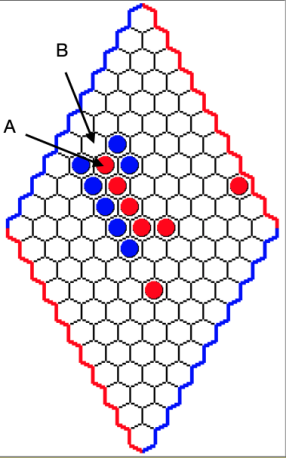
\includegraphics[scale=0.5]{3.png}
    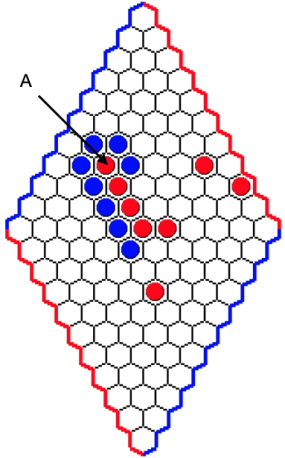
\includegraphics[scale=0.5]{4.png}
\end{figure}


Notre stratégie est efficace et donne des résultats satisfaisants par rapport à sa simplicité puisqu'elle est basée sur le principe suivant : d'après une preuve de \textbf{David Gale} utilisant le \textbf{théorème de Brouwer}, pour le plateau hexagonal il existe toujours un gagnant (cf \textit{The Game of Hex and the Brouwer Fixed-Point Theorem}). Ainsi la stratégie de défense consiste à l'emporter en empêchant l'adversaire de construire son chemin.
\vspace{6pt}

\subsection{La stratégie Minimax}
Dans cette partie, nous avons voulu mettre en oeuvre une stratégie plus intelligente qui permettrait d'augmenter les chances de gagner la partie. Pour cela, nous nous sommes penchés sur les algorithmes Minimax qui semblent répondre à nos besoins. 
\subsubsection{Principe}
L'algorithme de Minimax est un algorithme récursif qui s'applique à la théorie des jeux à deux joueurs. Il consiste à maximiser les gains pour un joueur et les minimiser pour l'autre. À partir de chaque position, l'algorithme construit un arbre de jeu servant à prédire l'avenir.
\subsubsection{Implémentation}
\vspace{6pt}

Cette stratégie consiste à choisir le meilleur coup parmi les positions disponibles sur le plateau de jeu. En effet, notre joueur suit l'algorithme suivant :
\vspace{6pt}

\begin{algorithm}[H]
\caption{$Minimax Player$}
\begin{algorithmic}
\REQUIRE $G: graphe$
\STATE $PossibleMoves \leftarrow getPossibleMoves(G)$
\STATE $n \leftarrow len(PossibleMoves)$
\STATE $Values \leftarrow [ ] * n$
\FOR{i\hspace{4pt} in\hspace{4pt} range(n)}
\STATE $Values[i] \leftarrow minimax(PossibleMoves[i])$
\ENDFOR
\STATE $Return \hspace{4pt} Max(Values, PossibleMoves)$
\end{algorithmic}
\end{algorithm}
La fonction Minimax utilisée dans cet algorithme consiste à optimiser la recherche du meilleur coup en limitant le nombre de nœuds visités dans l'arbre de jeu. Afin de réduire le nombre d'appels récursifs, il est possible de ne prendre en compte que les branches utiles au calcul en utilisant l'algorithme \textbf{Alpha-Beta}. Celui-ci prend en paramètre les variables suivantes :
\begin{itemize}
\item Node: la position où l'algorithme est appliqué.
\item MinMax: un booléen qui prend successivement les valeurs vrai et faux.
\item Depth: une variable qui limite la hauteur de l'arbre d'appel de cette fonction.
\end{itemize}

\begin{algorithm}[H]
\caption{$Minimax-Alpha-Beta$}
\begin{algorithmic}
\REQUIRE $node, alpha, betta, MinMax, depth$
\IF{$node \hspace{4pt}is\hspace{4pt} a \hspace{4pt}terminal\hspace{4pt} node \hspace{4pt} or\hspace{4pt} depth = 0\hspace{4pt} or \hspace{4pt} gameOver$}
\STATE $Return \hspace{4pt} Value(node)$
\ELSIF{$MinMax$}
\STATE $v\leftarrow +infini$
\FOR{$each\hspace{4pt}\hspace{4pt} child\hspace{4pt} of\hspace{4pt} the \hspace{4pt}node \hspace{4pt}$}
\STATE $v \leftarrow min(v, Minimax(child, alpha, beta, 1 - MinMax, depth - 1))$
\IF{$alpha >= v$}
\STATE $return \hspace{4pt} v$
\ENDIF
\STATE $beta \leftarrow  min(beta, v)$
\ENDFOR
\ELSE
\STATE $v\leftarrow -infini$
\FOR{$each\hspace{4pt}\hspace{4pt} child\hspace{4pt} of\hspace{4pt} the \hspace{4pt}node  \hspace{4pt}$}
\STATE $v \leftarrow max(v, Minimax(child, alpha, beta, MinMax, depth - 1))$
\IF{$v >= beta$}
\STATE $return \hspace{4pt} v$
\ENDIF
\STATE $beta \leftarrow  max(beta, v)$
\ENDFOR
\ENDIF
\STATE $Return \hspace{4pt} v$
\end{algorithmic}
\end{algorithm}
\vspace{8pt}


L'algorithme Minimax visite le graphe de jeu pour faire remonter à la racine une valeur qui est calculée récursivement à partir de la valeur initiale de chaque noeud, cette valeur représente la qualité de la position. En effet, l'évaluation de cette position consiste d'abord à trouver le plus court chemin vers un bord de la table de jeu et qui a la même couleur du joueur, à travers l'algorithme de Djisktra qui est expliqué en-dessous. Ensuite, la qualité de ce chemin pour le joueur est mesuré en comptant le nombre de positions disponibles dans le graphe. Finalement, la qualité globale de la position est la différence entre la qualité de cette position liée au premier joueur et au deuxième.
L'algorithme de Djikstra calcule la distance minimale entre deux points sans prendre en compte leur nature. Nous avons, donc légèrement modifié cet algorithme afin de prendre en compte les cases de la couleur de l'adversaire en modifiant le poids des arêtes selon la couleur de ces cases. Enfin, le résultat calculé est un chemin minimal entre la position actuelle et une position quelconque du bord associé à la même couleur.

Cette stratégie a prouvé son efficacité contre la stratégie du bloqueur, cependant la complexité de cette méthode est élevée car elle fait des appels récursifs sur tous les points disponibles du graphe, ce qui produit une valeur au voisinage de \textbf{O(vertices * depth) * C}, avec \textbf{C} la complexité de l'algorithme de Djikstra qui est égale à \textbf{O(a + n*log(n))} (a = arcs, n = sommets).

\subsection{La méthode de Kirchhoff}
\vspace{4pt}

Cette stratégie implémente la méthode des résistances, celle du chapitre 3 de l'article d'Anshelevich \textit{The Game of Hex: An Automatic Theorem Proving Approach to Game
Programming}.
\vspace{1pt}

\subsubsection{Principe}
Le plateau de jeu est assimilé à un dipôle relié à un générateur de tension. De plus, à chaque case du graphe est associée une valeur de résistance.
En utilisant ces résistances, nous allons calculer la résistance totale du plateau pour les deux joueurs, et en faire le rapport. Parmi toutes les cases jouables, celle dont le rapport des résistances est minimal sera la case choisie par le joueur noir, et inversement pour le joueur blanc. 

Le calcul des résistances totales s'effectue en résolvant un système linéaire.

\subsubsection{Mise en équation}
Tout d'abord nous associons à chaque case du graphe une résistance de valeur : 
\vspace{4pt}

\noindent\textit{Du point de vue du circuit noir}
\vspace{4pt}

\begin{itemize}
    \item 1 si la case est vide
    \item 0 si la case est occupé par le joueur noir
    \item $+\infty$ si la case est occupée par le joueur blanc
\end{itemize}
\vspace{4pt}

\noindent\textit{Du point de vue du circuit blanc}
\begin{itemize}
    \item 1 si la case est vide
    \item 0 si la case est occupé par le joueur blanc
    \item $+\infty$ si la case est occupée par le joueur noir
\end{itemize}

\ \\
\indent En pratique, nous avons initialement fixé les résistances infinies à $1000$ et les résistances nulles à $0.001$. Cependant suite à des problèmes d'overflow lors de la résolution du système pour de grands plateaux de jeu, nous les avons fixées respectivement à $2$ et $0.5$.
\vspace{4pt}

Ensuite il est nécessaire de définir le concept de résistance adjacente entre deux cases, une telle résistance vaut la somme des résistances des deux cases incidentes.
Ainsi, pour mettre en place nos équations, nous avons schématisé notre graphe comme étant un circuit électrique, chaque sommet représentant un noeud et chaque résistance étant située entre deux sommets adjacents. Nous avons ensuite mis artificiellement un générateur de tension entre un sommet d'une couleur du pôle nord du circuit et un sommet de la même couleur du pôle sud. Une telle modélisation nous a permis d'effectuer la méthode des mailles et obtenir une équation pour chaque maille élémentaire.
Par exemple, avec 3x3 sommets :

\begin{figure}[H]
    \centering
    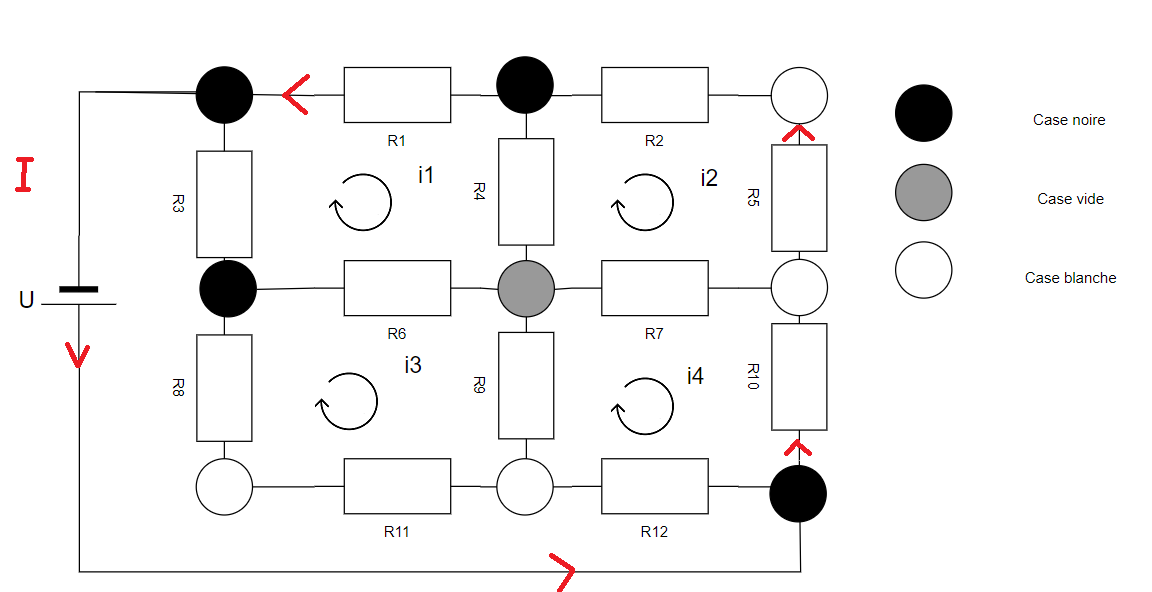
\includegraphics[width = 13cm]{resistance.png}
    \caption{Modélisation du graphe en circuit électrique}
    \label{circuit}
\end{figure}
\noindent Ainsi nous obtenons 5 mailles, donc 5 équations :\\
\indent $i_1(R_1+R_3+R_4+R_6)-i_2R_4-i_3R_6=0$\\
\indent $i_2(R_2+R_4+R_5+R_7)-i_4R_7-i_1R_4=0$\\
\indent $i_3(R_6+R_8+R_9+R_{11})-i_4R_9-i_1R_6=0$\\
\indent $i_4(R_7+R_9+R_{10}+R_{12})-i_3R_9-i_2R_7=0$\\
\indent $I(R_1+R_2+R_5+R_{10})-i_1R_1-i_2(R_2+R_8)-i_4R_{10}=U$

Nous obtenons 5 équations et 5 inconnues, le système admet alors une unique solution. Il ne reste plus qu'à résoudre ce système.

\subsubsection{Résolution du système linéaire}

Pour résoudre le système linéaire, avons utilisé un algorithme de pivot de Gauss. Cependant, étant confrontés à des problèmes \textbf{d'overflow}, nous avons été contraints de modifier les valeurs des résistances. Nous avons également changé le type des variables du système en \lstinline{double} au lieu de \lstinline{float}. \\
Ayant un grand nombre de coefficients nuls dans le système d'équations, nous aurions pu réduire la complexité de cette résolution en utilisant les matrices creuses de la bibliothèque GSL. Cependant, nous n'y avons pas pensé dès le départ et nous aurions opéré le changement si nous avions eu plus de temps.

\subsubsection{Calcul du score}
Pour calculer le score il est nécessaire de calculer deux résistances : la résistance totale noire et la résistance totale blanche liés à un coup donné. Le rapport $E=\frac{Resistance\_noire}{Resistance\_blanche}$ nous donne des informations sur le caractère avantageux du coup. Plus E est petit et plus le joueur noir est avantagé tandis que plus E est grand, plus le joueur blanc est avantagé. Ainsi, à chaque tour du joueur, il calculera ce rapport pour chaque case et il choisira pour coup celui offrant le meilleur score. Si ce rapport vaut 0, c'est que le joueur noir a gagné. 

%\subsubsection{Recherche du meilleur coup}
%Dans l'optique de trouver le coup le plus avantageux, le joueur va calculer le score lié à tous les coups possibles. Il choisit ensuite le coup associé au score le plus avantageux. Cela correspond au score $E$ minimal si sa couleur est le noir ou maximal sinon.

\subsubsection{Complexité de la recherche} 
Afin d'évaluer la complexité de la fonction \lstinline{play} de \textcolor{red}{joueur\_resistance.c}, il est nécessaire de connaître celle des fonctions intervenant lors du calcul des résistances.
 \lstinline{generate_meshes} initialise d'abord les éléments d'une matrice de taille \textbf{O(n)*O(n)} (la taille de la matrice varie selon la forme du plateau de jeu) en \textbf{O(n\up{2})} affectations ($n$ étant le nombre de sommets du graphe). Ensuite elle génère le système en \textbf{O(n\up{2})} autres affectations. Sa complexité en temps est donc de \textbf{O(n\up{2})}.
 
 Dans un premier temps, \lstinline{gauss} transforme ligne par ligne la matrice en un système triangulaire. Pour ce faire, on cherche le minimum en valeur absolue de la partie située sous la diagonale de chaque colonne en \textbf{O(n)} opérations, puis on fait l'opération de pivot en \textbf{O(n)} opérations. Comme il y a $n$ colonnes, cette étape est donc en \textbf{O(n\up{2})}. Ensuite, on résout le système triangulaire obtenu en \textbf{O(n\up{2})} opérations.
 
 Par conséquent, cette fonction admet une complexité en temps de \textbf{O(n\up{2})}. On pourra noter que la dimension exacte de la matrice considérée s'élève à $n+1$ pour une matrice carrée, contre $2*n + 1$ pour la matrice hexagonale, ce qui peut expliquer les différences de vitesse de jeu observées. Nous avons en effet constaté que le joueur mettait plus de temps à jouer sur un plateau hexagonal que sur un plateau carré.

\lstinline{get_ratio} initialise des vecteurs de taille $n$ en \textbf{O(n)} affectations. Puis elle appelle deux fois la fonction generate\_meshes, et deux fois \lstinline{gauss}. Enfin, elle libère la matrice du système ligne par ligne, donc en \textbf{O(n)} opérations. Sa complexité en temps s'élève donc à \textbf{O(n\up{2})}.\ \\

Ainsi, puisque la fonction \lstinline{play} appelle au plus $n$ fois \lstinline{get_ratio}, sa complexité en temps est en \textbf{O(n\up{3})}.

\subsubsection{Abaissement de la complexité}
Afin d'abaisser la complexité de l'algorithme choisissant le coup du joueur, nous avons décidé de limiter les coups à calculer. Lorsque l'adversaire choisit un mouvement, notre joueur ne considère que les cases voisines de ce mouvement pour le calcul des scores (le coup est dit de profondeur 1). Ainsi il ne considère pas toutes les cases du graphes pour le calcul du score, ce qui améliore la complexité mais diminue l'efficacité de la stratégie. Si aucune case voisine n'est disponible, il parcourt le graphe en prenant la première case disponible.

Ainsi lors d'un tour de jeu nous n'exécutons la fonction \lstinline{play} qu'un nombre constant de fois, ce qui fait passer la complexité d'un tour en \textbf{O(n\up{2})}.

\subsubsection{Conclusion sur la stratégie des résistances}
Si nous avions mieux géré la complexité avec ces systèmes d'équations creux en s'aidant de la bibliothèque GSL, nous aurions peut-être pu considérer toutes les cases du graphe pour cette stratégie. 

De plus, résoudre les problèmes d'overflow qui arrivaient lors de la résolution du système linéaire nous aurait permis d'employer des valeurs de résistances plus significatives. En effet, comme nos résistances, pourtant supposées infinies ou nulles, étaient très proches (facteur 4), les résistances totales obtenues variaient peu d'une case à l'autre, et des cases qui devaient être attrayantes ressortaient moins du lot. 
Par ailleurs, nous n'avons pu, par manque de temps, implémenter cette stratégie pour un graphe triangulaire. Ainsi la stratégie est ultimement moins efficace que ce que l'on espérait.

\section{Description des tests de validation}

\subsection{Tests unitaires}

Pour nous assurer du bon comportement de nos fonctions, il a été nécessaire de les tester. En ce qui concerne le \lstinline{graph_t}, nous avons dû vérifier que ses matrices d'adjacence et de couleur étaient bien initialisées, ou encore que la fonction \lstinline{is_winning} reconnaissait bien les graphes gagnants et que sa pile fonctionnait bien. Cependant, pour des matrices de taille élevée, il est fastidieux de vérifier leurs éléments un à un. Nous avons donc également utilisé des fonctions d'affichage pour vérifier que les éléments des matrices étaient corrects.

D'autres tests ont concerné le calcul des résistances liés à la stratégie de Kirchhoff. Il a en effet fallu s'assurer que les systèmes linéaires étaient bien construits, que notre méthode de Gauss fonctionnait ou encore que les cases les plus avantageuses (typiquement celles qui débouchent sur une victoire) étaient choisies avant les autres.

Nous avons eu recours dans ce projet à l'implémentation de deux types abstraits de données (\textbf{TAD}): une pile et un tableau dynamique. Afin de s'assurer de leur bon fonctionnement, nous avons mis en place des tests structurels. Par exemple, pour tester la fonction \lstinline{empty__dynamic_array}, nous avons vérifié si la taille du tableau créé était égale 0. Puis nous ajoutions un autre élément et nous vérifions si la capacité avait bien doublé et si le nombre d'éléments avait été incrémenté.

\subsection{Tests de fuites mémoire}
Tester la gestion de la mémoire de notre programme a été nécessaire pour ce projet. Pour cela, nous avons utilisé \textbf{Valgrind} pour vérifier notre code.
\subsection{Test de pré-commit}
Afin de s'assurer que nos commit respectent les tests utilisés sur la forge, nous avons écrit un script qui s'exécute automatiquement après chaque commit. Cela permet de rejeter les modifications si les tests échouent. 
\subsection{Couverture des tests}

Afin d'estimer la couverture de notre code par ces tests, nous avons utilisé l'outil \textbf{gcov}. Cela nous permet de savoir quelles lignes de chaque fichier sont exécutées lors des tests, et d'améliorer ceux-ci en conséquence. On pourra noter que certains fichiers sont moins couverts que d'autres, cela s'explique par le fait que nous ne lançons pas les fonctions d'affichage y étant définies lors de nos tests (par exemple pour \textcolor{red}{graph.c}).

\section{Conclusion} 
Comme attendu, la stratégie aléatoire perd presque systématiquement contre les autres. Elle l'emporte parfois face à la stratégie de Kirchhoff puisque cette dernière a été allégée pour gagner en complexité. Notre algorithme le plus efficace pour l'emporter est finalement celui qui repose sur "Minimax".
Ce projet nous a finalement offert l'occasion de mettre en application les connaissances acquises au cours du second semestre, comme par exemple l'utilisation de bibliothèques dynamiques, d'outils de déboguage puissants comme \textbf{gdb}, ou encore une nouvelle méthode pour renforcer les tests avec \textbf{gcov}. Les cours d'algorithmique des graphes ont également été sollicités pour mener le projet à bien notamment par l'utilisation de parcours en profondeur et de la manipulation de la connexité des graphes pour l'implémentation des stratégies.

\label{LastPage}
\end{document}
